\documentclass{article}
\usepackage[margin=1.0in]{geometry}
\usepackage{graphicx}
\usepackage{paralist}
\usepackage{listings}
\usepackage{hyperref}
\usepackage{amsthm}
\usepackage{amsmath}
\usepackage{amsfonts}
\usepackage{amssymb}
\usepackage{anyfontsize}
\usepackage[usenames,dvipsnames]{xcolor}

\theoremstyle{definition}
\newtheorem{example}{Example}[section]
\newtheorem{definition}{Definition}[section]
\renewcommand\lstlistingname{Figure}

\lstdefinelanguage{ets}
{
morekeywords={->,True, False},%
keywords={->,--->,<---,True, False},%
alsoletter={-,>,<},
morecomment=[l]\#,%
commentstyle=\color{red}\ttfamily,
%backgroundcolor=\color{gray!10},
keywordstyle=\color{blue}\bfseries,
numbers=left,
basicstyle=\footnotesize\ttfamily,
numberstyle=\small\ttfamily,
numbersep=1.5em,
showstringspaces=false,
breaklines=false,
frame=lines,
%framexleftmargin=2.5em,
xleftmargin=2.5em,
}

\lstdefinelanguage{sts}
{
morekeywords={True, False, VAR, OUTPUT, TRANS, DEF, INIT, INVAR},%
morecomment=[l]\#,%
commentstyle=\color{red}\ttfamily,
%backgroundcolor=\color{gray!10},
keywordstyle=\color{blue}\bfseries,
numbers=left,
basicstyle=\footnotesize\ttfamily,
numberstyle=\small\ttfamily,
numbersep=1.5em,
showstringspaces=false,
breaklines=false,
frame=lines,
%framexleftmargin=2.5em,
xleftmargin=2.5em,
}

\lstdefinelanguage{Ini}
{
    basicstyle=\ttfamily\small,
    columns=fullflexible,
    tag=[s]{[]},
    tagstyle=\color{Orchid}\bfseries,
    usekeywordsintag=true,
    morecomment=[l]{;},
    commentstyle=\color{gray}\ttfamily,
    alsoletter={=},
    ndkeywords={=},
    ndkeywordstyle=\color{green}\bfseries,
numbers=left,
numbersep=1.5em,
showstringspaces=false,
breaklines=false,
frame=lines,
%framexleftmargin=2.5em,
xleftmargin=2.5em
}[html]

\begin{document}

\title{\vspace{5cm}{\fontsize{70}{70}\selectfont \textbf{CoSA}}\\ \vspace{1cm}User Manual}
\author{\\ \\ \\ \\ \textbf{Cristian Mattarei}}

\maketitle

\newpage
\tableofcontents

\newpage
\section*{Introduction}

CoSA is a symbolic model checker for hardware design. It incorporates
a variety of state-of-the-art techniques to achieve performance, while
providing a simple and intuitive interface. This document describes
all functionalities provided by CoSA, and the description is supported
by a series of running examples.

\section{Overview}

The main inputs to CoSA to define a model checking
(\textsection~\ref{sec:model_checking}) verification task are:
\begin{itemize}
\item a list of comma-separated input files
  (\textsection~\ref{sec:input_formats}) describing the hardware;
\item a verification problem
  (\textsection~\ref{sec:problem_definition}) e.g.; safety
  (\textsection~\ref{sec:safety_and_ltl}), LTL
  (\textsection~\ref{sec:safety_and_ltl}), or equivalence checking
  (\textsection~\ref{sec:equivalence_checking}); and
\item a property (\textsection~\ref{sec:properties}).
\end{itemize}

\noindent
The other parameters can be divided into:
\begin{itemize}
\item encoding options (\textsection~\ref{sec:encodings});
\item performance optimizations parameters
  (\textsection~\ref{sec:optimizations}); and
\item debugging (\textsection~\ref{sec:debugging}).
\end{itemize}

\noindent
The results of the analyses, as counterexample traces, are provided in
multiple formats (\textsection~\ref{sec:results_analysis}).

\

\noindent
All these options can be either provided as parameters to CoSA on the
command line, or as a single problem file
(\textsection~\ref{sec:problem_file}).

\

\noindent
For more information on the actual parameters, run CoSA with
\texttt{-h}.


\section{Background}
This section provides an overview of the formal aspects at core of
CoSA, and it is intended for the users that are not familiar with
symbolic model checking and formal verification.

\subsection{Model checking}
\label{sec:model_checking}
Model checking is a technology that allows for an efficient and
exhaustive testing of a system. Model checking can be applied to
different domains, and the common problem this technique can solve is
to prove that a system - in our case a hardware design - meets a set
of predefined and expected behaviors, usually represented as system
assertions. A model checking problem is usually denoted as $M \models
\varphi$, where $M$ is a mathematical representation of the system,
and $\varphi$ is the expected behavior. For instance, given a hardware
component \emph{Sum} that computes the sum of its input ports $I_1$
and $I_2$, and that provides the result to the output $O$, a
conventional testing procedure for \emph{Sum} would require to check
that if $I_1=0$ and $I_2=0$ then $O=0$, and that $I_1=1$ and $I_2=0$
results into $O=1$, and so on. However, with model checking we can
directly evaluate if \emph{Sum} $ \models (O=I_1+I_2)$, and if this is
not the case the model checker (such as CoSA) will provide a
counterexample to the expected behavior (i.e., $O=I_1+I_2$), which is
represented as a series of assignments to the ports such as $I_1=16,
I_2=13, O=32$.

Model checking is a fundamental technology when developing complex
systems, thus over the years multiple different techniques have been
developed to efficiently solve the problem. A major distinction is
between symbolic and explicit state (model checking), and the
different resides in the technique used to represent the system. 

\subsection{Symbolic transition system}
\label{sec:sts}

CoSA, being a symbolic model checker, converts all the input models
into an internal representation that is called Symbolic Transition
System (STS). An STS has an established semantics, and we report its
definition in \ref{def:sts}. Intuitively, an STS is composed of a set
of variables, a formula that defines the initial state of the system,
and a transitional relation formula that defines how the system
evolves. 


\begin{definition}[Symbolic Transition System]
\label{def:sts}
A \emph{Symbolic Transition System} is a tuple $S = \langle V, I,
T\rangle$ where $V$ is a set of (input $V_I$, state $V_S$, and
output $V_O$) variables, $I(V)$ is a formula representing the initial
states, and $T(V, V')$ is a formula representing the transitions.  A
\emph{state} of $S$ is an assignment to the variables $V_S$.
\end{definition}

\begin{example}[STS clock behavior encoding]
  \label{sts:clock_beh}
Given a clock signal that starts from 0, and keeps oscillating at
every step, its representation would be a tuple $STS_c := \langle V_c,
I_c, T_c\rangle$ where:
\begin{itemize}
\item $V_c := \{\text{clk}\}$,
\item $I_c := \{\text{clk} = 0\}$,
\item $T_c := ((\text{clk} = 0) \rightarrow (\text{clk}' = 1)) \wedge$

~~~~~~~~$((\text{clk} = 1) \rightarrow (\text{clk}' = 0))$.
\end{itemize}


The symbols with $'$ (e.g., $\text{clk}'$) are called primed variable,
and they represent the value after the transition. For instance, the
formula $(\text{clk} = 0) \rightarrow (\text{clk}' = 1)$ states that
if clk = 0 before the transition, then clk should be equal to 1 after
the transition.
  
\end{example}

The STS representation is important in CoSA because it allows the user
to define complex behavior interaction via synchronous products with
other systems. Its definition is reported in \ref{def:sync}.

\begin{definition}[Synchronous Product of STS]
  \label{def:sync}
  Given two Symbolic Transition Systems $S_1 := \langle V_1, I_1,
  T_1\rangle$ and $S_2 := \langle V_2, I_2, T_2\rangle$ where $V_1
  \cap V_2 = \emptyset$, the synchronous product $S$ of $S_1$ and
  $S_2$, namely $S_1 \times S_2$, is defined as $S := \langle V_1 \cup
  V_2, I_1 \wedge I_2, T_1 \wedge T_2 \rangle$.
\end{definition}

\begin{example}[Synchronous product of STSs]
This example shows how the synchronous product can be used to
integrate multiple systems. We start to introduce a counter that goes
from 0 to 3 at every posedge of ``clk'', defining it with the tuple
$STS_3 := \langle V_3, I_3, T_3\rangle$ where:
\begin{itemize}
\item $V_3 := \{\text{output}, \text{clk}\}$,
\item $I_3 := \{\text{output} = 0\}$,
\item $T_3 := (((\text{clk} = 0) \rightarrow (\text{clk}' = 1)) \rightarrow $

~~~~~~~~~~~~~$(((\text{output} < 3) \rightarrow (\text{output}' = \text{output} +
  1)) \wedge$

~~~~~~~~~~~~~$((\text{output} \geq 3) \rightarrow (\text{output}' = 0)))) \wedge$

~~~~~~~~$(\neg((\text{clk} = 0) \rightarrow (\text{clk}' = 1)) \rightarrow$

~~~~~~~~~~~~~$(\text{output}' = \text{output}))$.
  
\end{itemize}

We can notice that the $STS_3$ does not constraint the behavior of
``clk'', and it is used only used in the transition relation to
defined the behavior of the variable ``output'', and in principle, the
counter can provide the value 0 forever if the clock does not
oscillate. The synchronous product between $S_3$ and $S_c$ (defined in
the Example~\ref{sts:clock_beh}) integrates the formulae from both
systems, and it defines a composed STS that imposes the counter to
expose its expected behavior.

An important aspect of the synchronous products is that it may leads
to have deadlock states, usually from contradictory behaviors. For
instance, if $S_1 := \langle \{v\}, v = 0, \text{True}\rangle$ and
$S_2 := \langle \{v\}, v = 1, \text{True}\rangle$, the resulting $S_1
\times S_2$ will be $\langle \{v\}, \text{\textbf{False}},
\text{True}\rangle$, considering that $(v = 0) \wedge (v=1)$ is
contradictory.
  
\end{example}  

\subsection{Linear Temporal Logic (LTL)}
\label{sec:ltl}

Differently from safety verification (e.g., assertions), the Linear
Temporal Logic defines a behavior over system executions.  The syntax
of LTL is defined as follows:

$\varphi ::= p\ |\ \text{True}\ |\ \text{False}\ |\ \neg
\varphi\ |\ \varphi \wedge \gamma\ |\ \varphi \vee \gamma\ |\ \varphi
\rightarrow
\gamma\ |\ \text{\textbf{X}}(\varphi)\ |\ \text{\textbf{F}}(\varphi)\ |\ \text{\textbf{G}}(\varphi)\ |\ \varphi
\text{\textbf{U}} \gamma\ |\ \varphi \text{\textbf{R}} \gamma$

where:
\begin{itemize}
\item $p$ is an atomic proposition,
\item $\wedge$, $\vee$, $\rightarrow$, and $\neg$ are Boolean
  operators respectively for and, or, implies, and negation, and
\item \textbf{X}, \textbf{F}, \textbf{G}, \textbf{U}, and \textbf{R}
  are temporal operators:
\begin{itemize}
\item \textbf{G}lobally, e.g., $\text{\textbf{G}}(\varphi)$ means that
  $\varphi$ has to hold for every states,
\item \textbf{F}inally or Eventually, e.g.,
  $\text{\textbf{F}}(\varphi)$ means that $\varphi$ has to eventually
  hold,
\item ne\textbf{X}t, e.g., $\text{\textbf{X}}(\varphi)$ means that
  $\varphi$ has to hold at the next state,
\item \textbf{U}ntil, e.g., $\gamma \text{\textbf{U}} \varphi$ means
  that $\gamma$ has to hold until $\varphi$ becomes \emph{True},
\item \textbf{R}elease, e.g., $\gamma \text{\textbf{R}} \varphi$ means
  that $\varphi$ is \emph{True} until $\gamma$ becomes \emph{True}.
\end{itemize}
  
\end{itemize}

\begin{example}[Common LTL formalizations]
Following we report some common formalization examples:
\begin{itemize}  
\item ``the output value is always equal to 3'':
  
  $\text{\textbf{G}}(\text{output} = 3)$,
\item ``the output value will eventually reach 3'':

  $\text{\textbf{F}}(\text{output} = 3)$,
\item ``whenever there is a posedge reset, output should be equal to 0'':
  
  $\text{\textbf{G}}(((\text{rst} = 0) \wedge \text{\textbf{X}}(\text{rst} = 1)) \rightarrow \text{\textbf{X}}(\text{output} = 0))$,

\item ``at the first posedge reset, output should be equal to 0'':
  
  $\text{\textbf{F}}(((\text{rst} = 0) \wedge \text{\textbf{X}}(\text{rst} = 1)) \rightarrow \text{\textbf{X}}(\text{output} = 0))$,

\item ``the ready signal should always eventually be equal to 1'':
  
  $\text{\textbf{G}}(\text{\textbf{F}}(\text{ready} = 1))$,
  
\item ``every time that there is a send signal, eventually receive should hold'':
  
  $\text{\textbf{G}}(\text{send} \rightarrow \text{\textbf{F}}(\text{receive}))$.
  
\end{itemize}  
  
\end{example}


%% \subsection{Safety verification}
%% \label{sec:safety}

%% \subsection{Equivalence checking}
%% \label{sec:equivalence}


\section{Input formats}
\label{sec:input_formats}

CoSA supports multiple input formats, and while being equivalent from
an expressivity point of view, they are tailored and design to
accomplish different purposes. CoSA distinguish between different
formats by relying on their file extension. Running \texttt{CoSA -h}
shows the list of accepted input formats, and make sure that the
configuration is correct.

CoSA accepts a comma-separated list of files, and the resulting model
is \textbf{synchronous product} (\textsection~\ref{sec:sts}) between
all of them. This allows for a clear and explicit definition of
\textbf{reset procedures}, as well as environmental assumptions.

An input file can be provided with additional model flags listed in
squared brackets, which instruct the encoder of how to process the
file.

\begin{example}[Model flags]
   \texttt{CoSA -i input\_file.extension[model\_flag]} provides
   \texttt{input\_file.extension} as input file, with
   \texttt{model\_flag} as a model flag.
\end{example}


Following, we cover all the formats supported by CoSA.

\subsection{Verilog}
This format is natively supported by relying on PyVerilog, and it
requires a top-level model flag.

\begin{example}[Verilog input]
  \texttt{CoSA -i examples/counters\_4/counters\_4.v[Counters\_4]}
  provides \texttt{examples/ counters\_4/} \texttt{counters\_4.v} as input model,
  with \texttt{Counters\_4} as a top module.
\end{example}

\subsection{SystemVerilog}
SystemVerilog is supported using Verific, which is an industrial tool
that can translate SystemVerilog to Verilog. After translating the
file using Verific, CoSA relies on the internal Verilog encoder to
process the model. The SystemVerilog encoder also requires to provide
the top module as model flag.

\begin{example}[SystemVerilog input]
  \texttt{CoSA -i examples/counters\_4/counters\_4.sv[Counters\_4]}
  provides \texttt{examples/counters\_4/} \texttt{counters\_4.sv} as input model,
  with \texttt{Counters\_4} as a top module.
\end{example}

\subsection{CoreIR}
CoreIR~\cite{CoreIR} is supported by relying on PyCoreIR. Its file
extension is \texttt{.json}. The format accepts model flags to
instruct the encoder to extract additional information from the model
such as lemmas from CoreIR optimization passes \cite{cosa-paper}.

Currently, CoSA supports the following CoreIR model flags:
\begin{itemize}
\item \texttt{FC-LEMMAS}: it automatically extracts the lemmas from
  the fold constants CoreIR pass.
\end{itemize}

\begin{example}[CoreIR input with fold-constants lemmas]
  \texttt{CoSA -i examples/counters/counters.json} to load the
  \texttt{examples/counters/counters.json} design, or \texttt{CoSA -i
    examples/fold-constants/\\mpe\_fc.json[FC-LEMMAS]} to load
  \texttt{examples/fold-constants/} \texttt{mpe\_fc.json} with
  \texttt{FC-LEMMAS} as model flag.
\end{example}

\subsection{BTOR2}
BTOR2~\cite{btormc} is a very concise format to represent SMT-based
hardware designs. Its extension is \texttt{.btor} or \texttt{.btor2},
and it is mainly used to interface with other tools such as
Yosys~\cite{wolf2013yosys}, since it can produce such format.

\subsection{Symbolic Transition System (STS)}

This format allows for the definition of a component-based Symbolic
Transition System, which is characterized by:

\begin{itemize}
\item system variables, divided into \texttt{STATE}, \texttt{INPUT},
  \texttt{OUTPUT}, and \texttt{VAR}
\item initial states formula, i.e., \texttt{INIT}
\item transition relation formula, i.e., \texttt{TRANS}
\item invariant formula, i.e., \texttt{INVAR}, which constraints every
  states of the system, including the initial ones
\end{itemize}

The language supports also a typed modules definition and
instantiation. A module can be defined using the keyword \texttt{DEF}, followed
by a list of parameters, while its instantiation should be defined in
the \texttt{VAR} section.

Simple definition of an 8-bit counter with clock and reset is reported
in Figures \ref{counter-sts}, and \ref{counterh-sts}. The latter is
defined using sub-modules instantiation, and the lines that starts
with \texttt{\#} are comments.

\begin{lstlisting}[frame=single,language=sts,caption=Counter example,label=counter-sts]
VAR
clk: BV(1);
rst: BV(1);

OUTPUT
out: BV(8);

INIT
out = 0_8;
clk = 0_1;

TRANS
# Clock behavior definition
(clk = 0_1) <-> (next(clk) = 1_1);
# When posedge and not reset we increase out by 1
(posedge(clk) & ! posedge(rst)) -> (next(out) = (out + 1_8));
# When not posedge and not reset we keep the value of the out
(! posedge(clk) & ! posedge(rst)) -> (next(out) = (out));
# When reset we set out to 0
posedge(rst) -> (next(out) = 0);
\end{lstlisting}


\begin{lstlisting}[frame=single,language=sts,caption=Counter example (hierarchical),label=counterh-sts]
VAR
  clk: BV(1);
  rst: BV(1);
  counter_1: Counter(clk, rst);

OUTPUT
  out: BV(8);

TRANS
  # Clock behavior definition
  (clk = 0_1) <-> (next(clk) = 1_1);

INVAR
  # Enforcement of the equivalence between local output value
  # and the output of the sub-module
  out = counter_1.out;

DEF Counter(clk: BV(1), rst: BV(1)):
  VAR
  out: BV(8);

  INIT
  out = 0_8;

  TRANS
  # When posedge and not reset we increase out by 1
  (posedge(clk) & ! posedge(rst)) -> (next(out) = (out + 1_8));
  # When not posedge and not reset we keep the value of the out
  (! posedge(clk) & ! posedge(rst)) -> (next(out) = (out));
  # When reset we set out to 0
  posedge(rst) -> (next(out) = 0);
\end{lstlisting}


\subsection{Explicit state Transition System (ETS)}

This format allows for the definition of an Explicit States Transition System, which is characterized by two sections:
\begin{itemize}
\item states definition, expressed as values assignments to system
  variables, e.g., \texttt{I: clk = 0\_1} for the initial state or
  \texttt{S1: output = 4\_8} for the state S1, and so on
\item transitions definition, e.g., \texttt{I -> S1} defines a
  transition from the state I to the state S1
\end{itemize}

The language does not require types definitions, because they are
inferred by the values assignment. Figure~\ref{counter-ets} shows a an
example of a 2-bit counter, and the lines that starts with \texttt{\#}
are comments.

\begin{lstlisting}[frame=single,language=ets,caption=2-bit Counter,label=counter-ets]
# States definition
I: output = 0_2
S1: output = 1_2
S2: output = 2_2
S3: output = 3_2

# Transitions
I -> S1
S1 -> S2
S2 -> S3
S3 -> I
\end{lstlisting}

The ETS format is particularly suited for the definition of sequential
behaviors such as the \textbf{reset procedures}. In fact, most
hardware definitions require to be properly initialized before
performing any analysis. In the following example, the
\texttt{reset\_done} variable is used to keep track of the reset
status, and it is used to specify a pre-condition for the verification
properties.

\begin{lstlisting}[frame=single,language=ets,caption=Reset procedure example,label=reset]
I: rst = 0_1
I: reset_done = False

S1: rst = 1_1
S1: reset_done = False

SE: rst = 0_1
SE: reset_done = True

I -> S1
S1 -> SE
# the reset_done signal remains up forever, defined as a self-loop on the SE state
SE -> SE
\end{lstlisting}

\begin{example}[ETS input and synchronous product]
  \texttt{CoSA -i
    examples/counters\_4.v[Counters\_4],examples/\\counters\_4/rst\_beh.ets}
  to load the \texttt{examples/counters\_4.v} design and the ETS
  \texttt{examples/counters\_4/rst\_beh.ets} and perform a synchronous
  product between them.
\end{example}

\section{Properties}
\label{sec:properties}

CoSA supports the definition of invariant and Linear Temporal Logic
(LTL) properties. Moreover, the tool allows for the definition of
syntactic sugar and parametric generators. CoSA relies on
PySMT~\cite{gario2015pysmt} for the formulae management, thus the
syntax is going to related to this tool.

\subsection{Invariant}
An invariant property is a propositional formula over the system
variables that has to hold at any time. 

\begin{example}[Invariant property]
  Given the \texttt{examples/counters\_4.v} model, the invariant property
  \texttt{out < 10\_16} states that the value of \texttt{out} should
  be always less than the decimal encoding of \texttt{10} as a
  bit-vector of size {16}.
\end{example}

An invariant property can predicate also over the \texttt{next}
variables, which are the primed version of each variable.

\begin{example}[Invariant property with next]
  Given the \texttt{examples/counters\_4.v} model, the invariant property
  \texttt{(rst = 1\_1) -> (next(out) = 0\_16)} states that when the reset
  signal \texttt{rst} is equal to 1 (encoded as a bit-vector of size
  {1}), the primed value of \texttt{out} should be \texttt{0} (encoded
  as a bit-vector of size {16}).
\end{example}

\subsection{Linear Temporal Logic}
The support for LTL extends propositional logic with additional
temporal operators:
\begin{itemize}
\item \texttt{G}: for globally,
\item \texttt{F}: for finally/eventually,
\item \texttt{next}: for next,
\item \texttt{U}: for until,
\item \texttt{R}: for release.
\end{itemize}

\begin{example}[LTL property with Finally]
  Given the \texttt{examples/counters.json} model, the LTL property
  \texttt{F(self.out = 4\_16)} states that the signal
  \texttt{self.out} must reach the value \texttt{4} at some time in
  the future.
\end{example}

\begin{example}[LTL property with Finally Globally]
  Given the \texttt{examples/counters.json} model, the LTL property
  \texttt{F(G(self.out = 4\_16))} states that the signal
  \texttt{self.out} must reach the value \texttt{4} at some time in
  the future, and keep the value forever.
\end{example}

\begin{example}[LTL property with Globally Finally]
  Given the \texttt{examples/counters.json} model, the LTL property
  \texttt{G(F(self.out = 4\_16))} states that the signal
  \texttt{self.out} must reach the value \texttt{4} infinitely many
  times.
\end{example}


\subsection{Syntactic sugar}

In order to simplify the definition of hardware properties, CoSA
integrates an expandable support for syntactic sugar. Additional
syntactic sugars should be defined in \texttt{cosa/encoders/sugar.py},
and registered in \texttt{cosa/encoders/factory.py}. The one that are
registered can be seen in the \texttt{special operators} section of
the CoSA helper (parameter \texttt{-h}). Currently, CoSA supports the
following syntactic sugar:

\begin{itemize}
\item \texttt{posedge}, with a single
  parameter. \texttt{posedge(variable)} is equivalent to \texttt{(variable
    = 0\_1) \& next(variable = 1\_1)}, if \texttt{variable} is a
  bit-vector of size 1, while \texttt{(variable) \& next(! variable)} if
  \texttt{variable} is of Boolean type,
\item \texttt{negedge}, which is implemented as \texttt{posedge} with
  inverted polarity,
\item \texttt{change}, with a single
  parameter. \texttt{change(variable)} is equivalent to
  \texttt{(variable != next(variable)},
\item \texttt{nochange}, with a single
  parameter. \texttt{nochange(variable)} is equivalent to
  \texttt{(variable = next(variable)},
\item \texttt{ones}, with a single parameter. \texttt{ones(variable)}
  provides the highest possible value of \texttt{variable},
\item \texttt{zero}, with a single parameter. \texttt{zero(variable)}
  provides the bit-vector encoding of all zeros, given the size of
  \texttt{variable},
\item \texttt{dec2bv}, with a two parameters. \texttt{dec2bv(value,
  variable)} provides the bit-vector encoding of value, given the size
  of \texttt{variable}.
\end{itemize}

\subsection{Generators}

More complex behaviors sometimes require the definition of parametric
modules to support the verification. The generators help on
simplifying those properties, by providing a parametric way to defined
commonly used symbolic transition systems. A common example of a
generator is the definition of a \emph{scoreboard} to verify the
behavior of a \emph{FIFO}. The purpose of a \emph{scoreboard} is to
keep track of a packet that goes into the \emph{FIFO}, and tells when
it is supposed to come out, according with the number of pushes and
pops that have been performed. An approach to define such behavior
would be to define an STS that models the \emph{scoreboard}, which in
synchronous product with the original system would allow the user to
specify the appropriate property. However, with the CoSA generators
this verification is much simpler.

\begin{example}[Generators usage]
  Given the FIFO implementation in \texttt{examples/fifo/fifo.sts},
  the property that verify its behavior is defined as \texttt{sb.end
    -> (sb.packet = output)} by instantiating the generator
  \texttt{sb=FixedScoreboard} \texttt{(input, 6, posedge(clk))}. The meaning of
  the property is that when signal \texttt{end} from the
  \emph{scoreboard} \texttt{sb} is \emph{True}, then the
  \texttt{packet} should be equivalent to the \texttt{output} of the
  \emph{FIFO}. While the instantiation of the \emph{scoreboard} takes
  as input the \texttt{input} of the \emph{FIFO}, its length (in this
  case is 6), and the signal that triggers the coming of a new packet.
\end{example}

The generators can be defined in \texttt{cosa/encoders/generators.py}
and should be registered in \texttt{cosa/
  encoders/factory.py}. CoSA
currently provides this set of generators:

\begin{itemize}
\item \texttt{FixedScoreboard}: \emph{scoreboard} for a FIFO with no
  pop. The parameters are (input\_port, max\_value, push\_signal), and
  its values are (end, tracking),
\item \texttt{Scoreboard}: \emph{scoreboard} for a FIFO with push and
  pop. The parameters are (input\_port, max\_value, push\_signal,
  pop\_signal), and its values are (end, tracking),
\item \texttt{Random}: provides a non-deterministic value. The
  parameter is (size) and its value is (value), and it can be either a
  variable (it would consider its size), or a decimal value.
\end{itemize}  

\section{Verification definition}
\label{sec:problem_definition}

This section covers the definition of a verification task, including
the environmental behavior where the system design is supposed to
operate.

\subsection{Environmental assumptions}

A circuit usually requires to be analyzed assuming a specific
environmental behavior. This might include clock behaviors, reset
procedures, and valid inputs configurations. This set of assumptions
can be set relying on additional models defined using STSs or ETSs and
include them in the list of input files. However, CoSA provides also a
set of automated procedures to add environmental behaviors. Currently,
the tool supports automated clock definition.

\begin{figure}[ht]
  \centering
    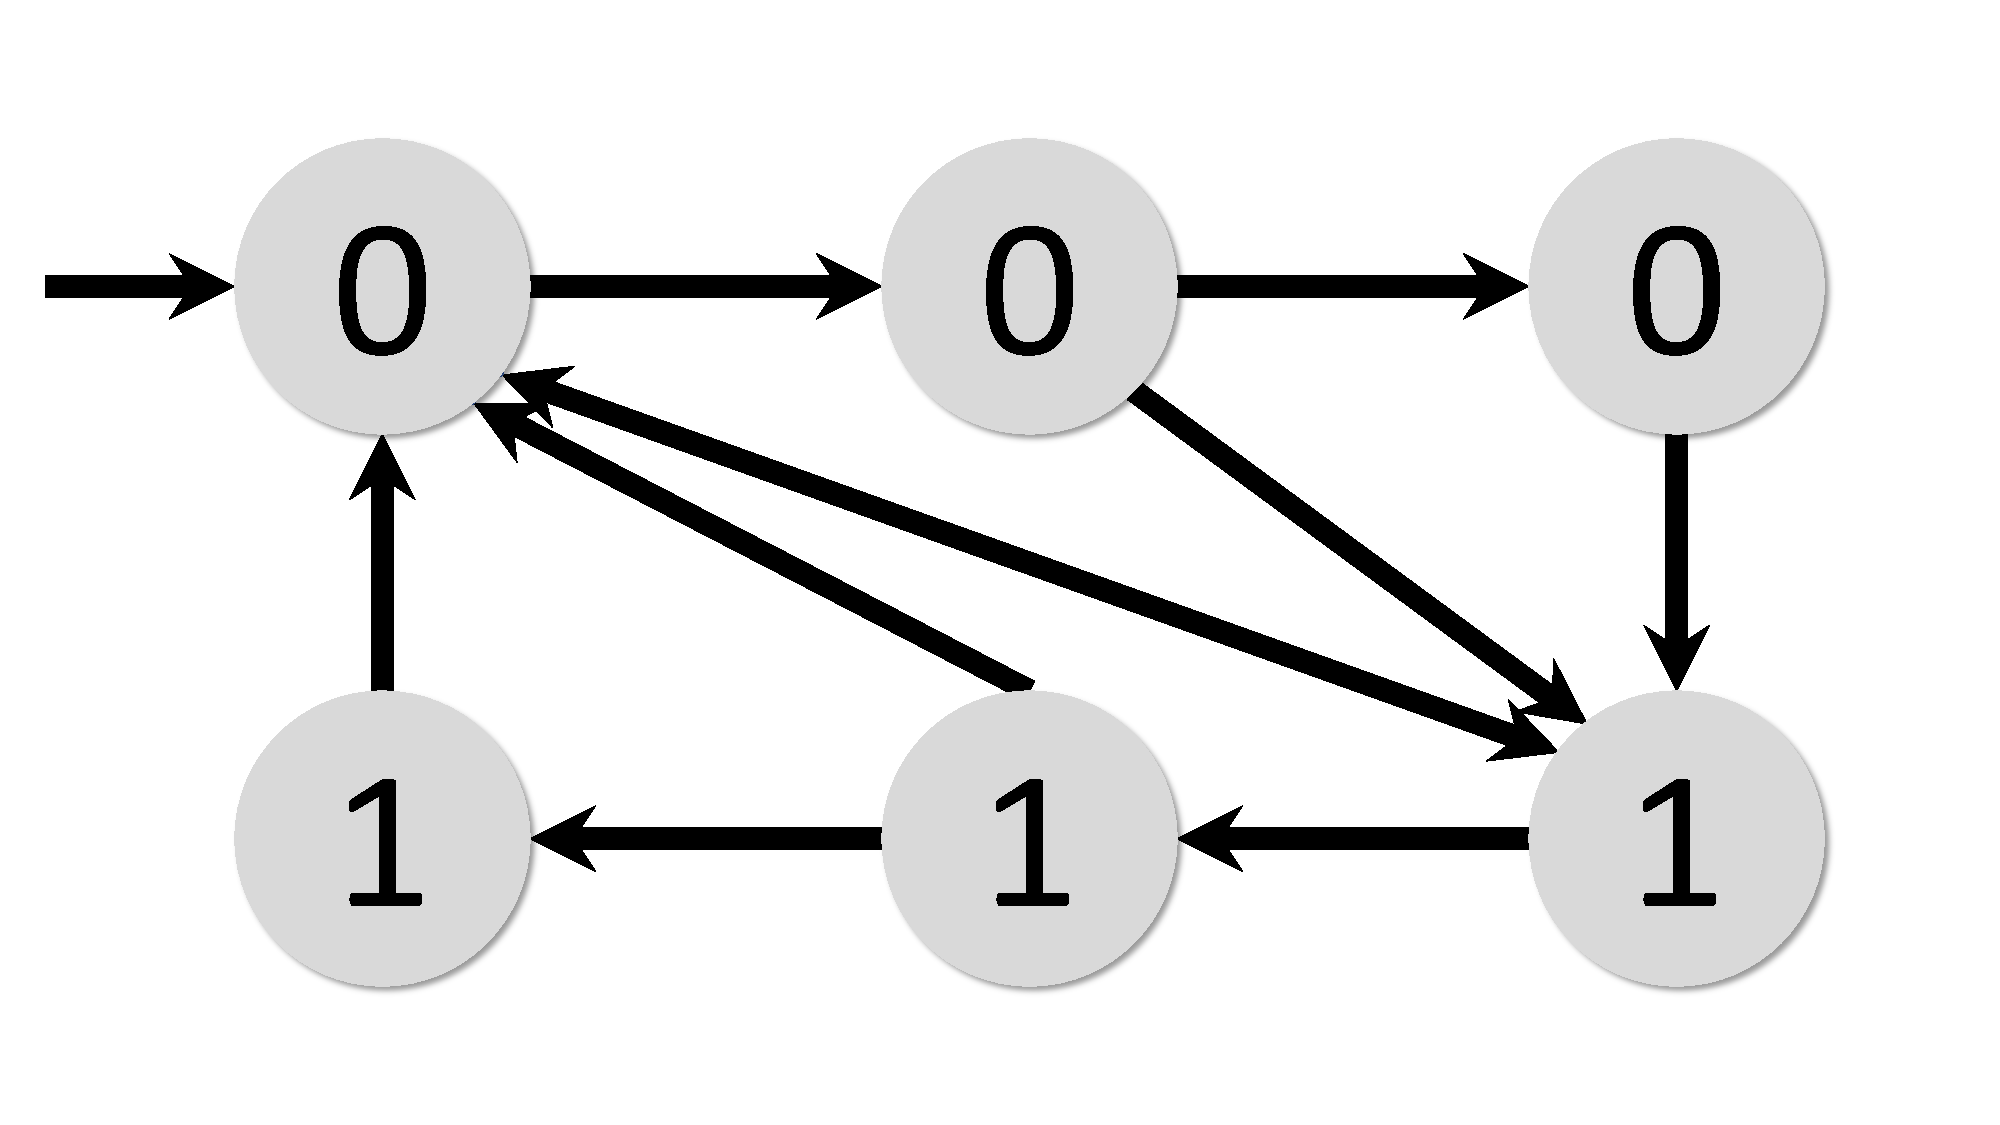
\includegraphics[width=0.4\textwidth]{img/NonDetClock.pdf}
    \caption{Non-deterministic clock behavior of period = 3}
    \label{fig:nondet_clock}
\end{figure}

The parameter \texttt{--add-clock} links a clock behavior to each
input signals whose name contains the ``clk'', and their behavior is
defined by the parameter \texttt{--clock-behaviors}. Clock behaviors
can be defined in the file \texttt{cosa/encoders/clock.py} and should
be registered in the file
\texttt{cosa/encoders/factory.py}. Currently, CoSA supports the
following clock behaviors:

\begin{itemize}
\item \texttt{DetClock}: a deterministic behavior with fixed
  period. The parameters are (clock\_variable, period), and it will
  generate a behavior that oscillates from 0 to 1, keeping its value
  constant for period steps,
\item \texttt{ConstClock}: a constant behavior with fixed value. The
  parameters are (clock\_variable, value), and it will keep the value
  forever. This is usually used with clock abstraction (see
  Section~\ref{sec:optimizations}),
\item \texttt{NondetClock}: a non-deterministic behavior with maximum
  period. The parameters are (clock\_variable, period), and it will
  generate a behavior that oscillates from 0 to 1, keeping its value
  constant for at most period steps. Figure~\ref{fig:nondet_clock}
  shows the transition system of a non-deterministic clock with period
  = 3.
\end{itemize}

If \texttt{--clock-behaviors} is not defined, the default
configuration is reported in Table~\ref{tab:clock_default}.

\begin{table}[h]
  \centering
\begin{tabular}{ c c | l }
  \# of clock signals & clock abstraction & \multicolumn{1}{c}{clock behaviors} \\ \hline 
  1 & No & \texttt{DetClock}, period = 1 \\
  ~~~$>1$ & No & \texttt{NondetClock}, period = 3  \\
  1 & Yes & \texttt{ConstClock}, value = 0 or 1 \textbf{*}\\
  ~~~$>1$ & Yes & \texttt{ConstClock}, value = 0 or 1 \textbf{*} \\
  \\
  \multicolumn{3}{l}{\textbf{*}: 1 if its behavior is defined only on posedge, 0 otherwise}
\end{tabular}
\caption{Default clock behaviors}
\label{tab:clock_default}
\end{table}


\subsection{Simulation}
The simulation generates a system execution of a provided depth. This
verification does not require a property, in that case it will be set
to \emph{True}. If a property is provided the shortest execution
reaching a state that satisfies the property is provided. If such a
state does not exist, the verification
fails. Table~\ref{tab:simulation_results} summarizes the possible
results of the analysis, given \texttt{bmc\_length} parameter.

\begin{table}[h]
  \centering
\begin{tabular}{ c c | c c }
  Property & Trace exists? & Result & Trace length \\ \hline 
  \emph{True} & Yes & \texttt{TRUE} & k+1  \\
  \emph{True} & No & \texttt{FALSE} & NA  \\
  $\varphi$ & Yes & \texttt{TRUE} & min(k) : $\varphi$  \\
  $\varphi$ & No & \texttt{FALSE} & NA  \\
\end{tabular}
\caption{Simulation results}
\label{tab:simulation_results}
\end{table}

\begin{example}[Simulation]
  Running \texttt{CoSA -i examples/counters/counters.sts --simulate}
  will generate a system execution of length equal to the default
  setting for the parameter \texttt{-k}, which is 10.
\end{example}

\subsection{Safety and LTL verification}
\label{sec:safety_and_ltl}

Safety (parameter \texttt{--safety}) and LTL (parameter
\texttt{--ltl}) verifications require to provide a property using the
parameter \texttt{-p}. An additional parameter \texttt{--prove}
requires the tool to try to prove that the property holds,
independently from the depth of the analysis (i.e.,
\texttt{--bmc\_length}/\texttt{-k} parameter). The result of the
analysis can be either \texttt{FALSE}, \texttt{TRUE}, or
\texttt{UNKNOWN}. The latter is provided when only a bounded proof
exists, and the probability to find an unbounded proof is dependent
from the depth of the analysis. Some input files can contain also
property definitions, and the usage of \texttt{--safety} or
\texttt{--ltl} parameter includes also those properties in the
verification task.  Table~\ref{tab:safety_results} summarizes the
possible results according with the parameter \texttt{--prove}, and
the existence of a proof.

\begin{table}[h]
  \centering
\begin{tabular}{ c c c c | c c }
  Property & Prove & Trace exists? & Proof found? & Result & Trace length \\ \hline
  $\varphi$ & Yes & Yes & NA & \texttt{FALSE} & min(k) : $\varphi$  \\
  $\varphi$ & Yes & No & Yes & \texttt{TRUE} & NA  \\
  $\varphi$ & Yes & No & No & \texttt{UNKNOWN} & NA  \\ \\
  $\varphi$ & No & Yes & NA & \texttt{FALSE} & min(k) : $\varphi$  \\
  $\varphi$ & No & No & NA & \texttt{UNKNOWN} & NA  \\
\end{tabular}
\caption{Safety and LTL results}
\label{tab:safety_results}
\end{table}

\begin{example}[Prove property]
  Running \texttt{CoSA -i examples/counters/counters.json --add-clock
    --safety\\ -p "count1.r.reg0.out < 19\_16"} performs a safety
  analysis of the property \texttt{count1.r.reg0.out < 19\_16}, and
  the result is shown in Figure~\ref{safety_unk}. While adding the
  parameter \texttt{--prove} to the command, CoSA is able to prove the
  property and it provides the result shown in Figure~\ref{safety_true}.

\begin{lstlisting}[frame=single,language=ets,caption=Safety example (UNKNOWN),label=safety_unk]
** Problem safety **
Result: UNKNOWN
BMC depth: 10
\end{lstlisting}

\begin{lstlisting}[frame=single,language=ets,caption=Safety example (TRUE),label=safety_true]
** Problem safety **
Result: TRUE
\end{lstlisting}

\end{example}


\subsection{Equivalence checking}
\label{sec:equivalence_checking}

The equivalence checking takes two systems and it verifies if they
start from the same initial state, and if they always receive the same
inputs they will always provide the same output. This verification
requires that the two systems have the same interface. The results of
this analysis is similar to the safety and LTL verification, and are
reported in Table~\ref{tab:equivalence_results}.

\begin{table}[h]
  \centering
\begin{tabular}{ c c c | c c }
  Prove & Trace exists? & Proof found? & Result & Trace length \\ \hline
  Yes & Yes & NA & \texttt{FALSE} & min(k) : $sys_1 \neq sys_2$  \\
  Yes & No & Yes & \texttt{TRUE} & NA  \\
  Yes & No & No & \texttt{UNKNOWN} & NA  \\ \\
  No & Yes & NA & \texttt{FALSE} & min(k) : $sys_1 \neq sys_2$  \\
  No & No & NA & \texttt{UNKNOWN} & NA  \\
\end{tabular}
\caption{Equivalence results}
\label{tab:equivalence_results}
\end{table}


\begin{example}[Equivalence checking]
  Running \texttt{CoSA -i examples/mul\_2/mul\_2.json --equivalence \\
    examples/mul\_2/mul\_2\_pe.json --prove -k 15} performs an
  equivalence checking between \texttt{examples/mul\_2/ mul\_2.json}
  and \texttt{examples/mul\_2/
    mul\_2\_pe.json}, and the result is
  shown in Figure~\ref{equivalence_unk}.

\begin{lstlisting}[frame=single,language=ets,caption=Equivalence example (UNKNOWN),label=equivalence_unk]
** Problem equivalence **
Result: UNKNOWN
BMC depth: 15
\end{lstlisting}

\end{example}

\subsection{Parametric model checking}

CoSA supports also parametric model checking analysis on extended
models. At the current stage, CoSA supports only to extend a model
with the internal model extension, which requires to select one of the
possible faulty behaviors using the parameter
\texttt{--model-extension}. The possible extension can be shown in the
CoSA helper (\texttt{CoSA -h}) under the section \texttt{model
  modifiers}. Additional modifiers can be defined in the
\texttt{cosa/modifiers/model\_extension.py} and should be registered
in \texttt{cosa/modifiers/factory.py}. At the current stage, CoSA
supports the following variable modifiers:

\begin{itemize}
\item \texttt{NonDeterministic}: allows for any possible value,
\item \texttt{Zero}: fixes the value to 0,
\item \texttt{High}: fixes the value to the highest possible value,
\item \texttt{Inverted}: inverts the correct value.
\end{itemize}

The result of a parametric model checking analysis is the region of
parameters (in this case the fault variables) that allow the system to
violate the property. As a precondition to this analysis, such
property should hold in the original model, otherwise the region of
parameters will be equal to \emph{True}. For instance, the property in
the Example~\ref{ex:param_nominal} holds for the given model, while
performing the parametric analysis on the extended model, as in the
Example~\ref{ex:param_extended}, it provides a region required to be
negated in order to satisfy the property. The parametric analysis is
also dependent to the parameter \texttt{--cardinality}, which provides
the upper bound of the number of failure that can occur in the system.

\begin{example}[Parametric verification (nominal analysis)]
  \label{ex:param_nominal}
  Running \texttt{CoSA -i
    examples/counters\_4/\\counters\_4.v[Counters\_4],examples/counters\_4/
    rst\_beh.ets --add-clock --safety -p "(reset\_performed \& !
    posedge(rst) \& posedge(clk)) -> ((next(out) < (out + 2\_16)))" -a
    "reset\_performed -> (rst = 0\_1);out < 240\_16" --prove --prefix
    trace} performs a safety analysis over the given model, property,
  and assumption, and the result is shown in
  Figure~\ref{parametric_safety_res}.

\begin{lstlisting}[frame=single,language=ets,caption=Safety analysis example,label=parametric_safety_res]
** Problem safety **
Result: True
\end{lstlisting}

\end{example}

\begin{example}[Parametric verification (faults analysis)]
\label{ex:param_extended}
  Running \texttt{CoSA -i
    examples/counters\_4/\\counters\_4.v[Counters\_4],examples/counters\_4/
    rst\_beh.ets --add-clock --model-extension High --parametric -p
    "(reset\_performed \& ! posedge(rst) \& posedge(clk))
    -> ((next(out) < (out + 2\_16)))" -a "reset\_performed -> (rst =
    0\_1);out < 240\_16" --prefix trace} performs a parametric model
  checking analysis extending the model with a \texttt{high} faulty
  behavior. The result is shown in Figure~\ref{parametric_res}, and
  the region three possible (minimal) assignments of cardinality 2.

\begin{lstlisting}[frame=single,language=ets,caption=Parametric analysis example,label=parametric_res]
** Problem parametric **
Result: UNKNOWN
BMC depth: 10
Region:
 - (counter_clk.out$FAILURE$ & counter_2.out$FAILURE$) or 
 - (counter_clk.out$FAILURE$ & counter_4.out$FAILURE$) or 
 - (counter_clk.out$FAILURE$ & counter_3.out$FAILURE$)
Executions: [1], [2], [3]
Traces (max) length: 4

*** TRACES ***

[1]:	trace[1]-parametric.txt
[2]:	trace[2]-parametric.txt
[3]:	trace[3]-parametric.txt
\end{lstlisting}

\end{example}

\section{Problem file}
\label{sec:problem_file}

In order to facilitate the usage of the tool in case of complex and
comprehensive analysis of a model, CoSA supports the definition of
problem files. In practice, a problem file links a model with a set of
formal analyses that have to be performed, and it is provided to the
tool with the parameter \texttt{--problems}.

Figure~\ref{problem_file} shows an example of a problem file, which is
composed of the following sections:
\begin{itemize}
\item \texttt{[GENERAL]}: it is required, and it defines the system
  model under analysis. A problem file accepts only one model, thus
  all encoding options have to be defined in this section. The files
  paths are local to the problem file, unless they start with
  \texttt{/} symbol,
\item \texttt{[DEFAULT]}: this section is optional, and it defines the
  default values of the verifications, in case they are not provided,
\item a list of verifications: each of them starts with a unique
  identifier in square brackets, and they set all the possible
  parameters that define the verification task.
\end{itemize}

Table~\ref{tab:general_section} lists the possible parameters for the
\texttt{[GENERAL]} section, while Table~\ref{tab:verification_section}
lists the parameters for the \texttt{[DEFAULT]} section and each
verification.

\begin{table}[h]
  \centering
\begin{tabular}{ l c c l c }
  Parameter & Default & & Parameter & Default \\ \cline{1-2} \cline{4-5}
abstract\_clock & False & ~~ & add\_clock & False \\
assume\_if\_true & False & ~~ & boolean & None \\
clock\_behaviors & None & ~~ & equivalence & None \\
model\_extension & None & ~~ & model\_file & None \\
run\_coreir\_passes & True & ~~ & symbolic\_init & False \\
vcd & False & ~~ & verbosity & None \\
zero\_init & None
\end{tabular}
\caption{\texttt{[GENERAL]} section options}
\label{tab:general_section}
\end{table}

\begin{table}[h]
  \centering
\begin{tabular}{ l c c l c }
  Parameter & Default & & Parameter & Default \\ \cline{1-2} \cline{4-5}
assumptions & None & ~~ & bmc\_length & 10 \\
bmc\_length\_min & 0 & ~~ & cache\_files & False \\
cardinality & -1 & ~~ & coi & False \\
description & None & ~~ & expected & None \\
formula & None & ~~ & full\_trace & False \\
generators & None & ~~ & incremental & None \\
lemmas & None & ~~ & precondition & None \\
prove & False & ~~ & smt2\_tracing & None \\
solver\_name & None & ~~ & strategy & None \\
time & False & ~~ & trace\_all\_vars & False \\
trace\_prefix & None & ~~ & trace\_values\_base & None \\
trace\_vars\_change & False & ~~ & vcd & False
\end{tabular}
\caption{\texttt{[DEFAULT]} and verification sections options}
\label{tab:verification_section}
\end{table}



\begin{lstlisting}[frame=single,language=Ini,caption=Problem file example,label=problem_file]
[GENERAL]
model_file: model.v[main_module]
add_clock: True

[DEFAULT]
bmc_length: 40

[safety_verification_1_id]
description: "Description of the safety verification 1"
formula: <property to be verified>
assumptions: <assumptions for the verification>
verification: safety
prove: True
expected: False

[safety_verification_2_id]
description: "Description of the safety verification 2"
...

[ltl_verification_1_id]
description: "Description of the LTL verification 1"
...

\end{lstlisting}

\begin{example}[Problem file definition]
The Figure~\ref{counter_problem} shows the problem file in
\texttt{examples/counter/problem.txt}, and it can be run with the
command \texttt{CoSA --problems examples/counter/problem.txt --prefix
  trace}.
  
\begin{lstlisting}[frame=single,language=Ini,caption=Problem file in \texttt{examples/counter/problem.txt},label=counter_problem]
[GENERAL]
model_file: counter.json,counter_live.sts
add_clock: True

[DEFAULT]
bmc_length: 40

[Globally]
description: "Globally Check"
formula: self.out < 4_16
assumptions: en_clr = 0_1 -> self.clr = 0_1
verification: safety
prove: True
expected: False

[Finally]
description: "Finally Check"
formula: F(self.out = 4_16)
assumptions: en_clr = 0_1 -> self.clr = 0_1
verification: ltl
prove: True
expected: True

[Liveness]
description: "Liveness Check"
formula: F(G(self.out = 4_16))
assumptions: en_clr = 0_1 -> self.clr = 0_1
verification: ltl
prove: True
expected: False
\end{lstlisting}

Figure~\ref{counter_problem_exec} shows the execution of the problem
file in Figure~\ref{counter_problem}. After performing the analysis,
CoSA provides a summary of the results, and it grabs the attention to
the analyses that have an unexpected result.

\begin{lstlisting}[frame=single,language=ets,caption=Analysis for the problem in Figure~\ref{counter_problem},label=counter_problem_exec]
Parsing file "examples/counter/counter.json"... DONE
Parsing file "examples/counter/counter_live.sts"... DONE
Solving "Globally" ... TRUE
Solving "Finally" ........ TRUE
Solving "Liveness" .............. FALSE

*** SUMMARY ***

** Problem Globally **
Description: "Globally Check"
Result: TRUE
Expected: FALSE
TRUE != FALSE <<<---------| ERROR

** Problem Finally **
Description: "Finally Check"
Result: TRUE
Expected: TRUE

** Problem Liveness **
Description: "Liveness Check"
Result: FALSE
Expected: FALSE
Counterexample: [1]
Trace length: 16

*** TRACES ***

[1]:	trace[1]-Liveness.txt

WARNING: Verifications with unexpected result
\end{lstlisting}

\end{example}

\begin{example}[Problem file definition (equivalence)]
The problem file reported in Figure~\ref{equivalence_problem} shows
the definition of an equivalence checking. In this case, the model
under analysis is the composition between \texttt{mul\_2.json}, and
\texttt{mul\_2\_pe.json}, thus all verifications are related to it.
  
\begin{lstlisting}[frame=single,language=Ini,caption=Problem file in \texttt{examples/mul\_2/problem\_1.txt},label=equivalence_problem]
[GENERAL]
model_file: mul_2.json
equivalence: mul_2_pe.json
add_clock: True

[DEFAULT]
bmc_length: 5

[Equivalence Checking]
description: "Mul2 is equivalent to Mul2 PE"
verification: equivalence
prove: True
expected: Unknown
\end{lstlisting}
\end{example}

\section{Results analysis}
\label{sec:results_analysis}

This section describes the information that CoSA produces after a
verification is performed.

\subsection{Counterexample traces}

The result of the verification can in some cases provide a
counterexample trace, which is an execution of the system that
supports the result of the analysis. CoSA produces finite-state
traces, but in case of LTL verification the trace can be infinite with
a lasso-shaped loop. CoSA can generate traces either in a human
readable textual format or in VCD format.

\subsubsection{Finite traces}

The format used by CoSA to represent traces is similar to the ETS
format (as shown in the Figure~\ref{simulation_trace}), and it
provides a series of states with assignments to the variables. The
default configuration shows only the top level \texttt{INPUT} and
\texttt{OUTPUT} ports, and all variables can be shown by using the
parameter \texttt{--trace-all-vars}. Moreover, a trace shows only the
variables that do not change their value, and this option can be
disabled with the parameter \texttt{--trace-vars-change}.

\begin{example}[Safety counterexample trace]
  Running \texttt{CoSA -i examples/counters\_4/\\counters\_4.v[Counters\_4] --simulate -k5}
  will generate a system execution of length equal to 6 (5 steps + initial state), as
  shown in Figure~\ref{simulation_trace}.

\begin{lstlisting}[frame=single,language=ets,caption=Simulation Counter\_4 ,label=simulation_trace]
** Problem simulation **
Result: TRUE
Execution:
---> INIT <---
  I: clk = 1_1
  I: out = 8_16
  I: rst = 1_1

---> STATE 1 <---

---> STATE 2 <---

---> STATE 3 <---

---> STATE 4 <---
  S4: clk = 0_1
  S4: rst = 0_1

---> STATE 5 <---
  S5: out = 0_16
  S5: rst = 1_1
\end{lstlisting}

\end{example}

\begin{example}[Counterexample with all variables]
  Running \texttt{CoSA -i
    examples/counters\_4/\\counters\_4.v[Counters\_4] --simulate -k5
    --trace-vars-change} will generate a system execution of length
  equal to 6 (5 steps + initial state), showing also the variables
  that change value, as shown in Figure~\ref{simulation_trace_change}.

\begin{lstlisting}[frame=single,language=ets,caption=Simulation Counter\_4 (with changing values),label=simulation_trace_change]
** Problem simulation **
Result: TRUE
Execution:
---> INIT <---
  I: clk = 1_1
  I: out = 8_16
  I: rst = 1_1

---> STATE 1 <---
  S1: clk = 1_1
  S1: out = 8_16
  S1: rst = 1_1

---> STATE 2 <---
  S2: clk = 1_1
  S2: out = 8_16
  S2: rst = 1_1

---> STATE 3 <---
  S3: clk = 1_1
  S3: out = 8_16
  S3: rst = 1_1

---> STATE 4 <---
  S4: clk = 0_1
  S4: out = 8_16
  S4: rst = 0_1

---> STATE 5 <---
  S5: clk = 1_1
  S5: out = 9_16
  S5: rst = 0_1
\end{lstlisting}

\end{example}


We can notice that state 5 differs between traces in Figures
\ref{simulation_trace} and \ref{simulation_trace_change}. In fact CoSA
does not guarantee a deterministic result in terms because the
internal solver can produce different models according with the state
space exploration that has been performed.

The parameter \texttt{--prefix} allows the user to save the trace to
file.

\begin{example}[VCD trace generation]
  Running \texttt{CoSA -i
    examples/counters\_4/counters\_4.v[Counters\_4] --simulate -k5
    --vcd --prefix trace} will generate a system execution of length
  equal to 6, and save it to a file with prefix ``trace'', as shown in
  Figure~\ref{simulation_trace_prefix}. A VCD trace is also generated
  when \texttt{--vcd} is set.

\begin{lstlisting}[frame=single,language=ets,caption=Simulation Counter\_4 (with prefix),label=simulation_trace_prefix]
** Problem simulation **
Result: TRUE
Executions: [1], [2]
Traces (max) length: 6

*** TRACES ***

[1]:	trace[1]-simulation.txt
[2]:	trace[2]-simulation.vcd
\end{lstlisting}

\end{example}



\subsubsection{Infinite traces}

The counterexample showing the violation of an LTL property usually
requires an infinite trace. For instance, if the property $F(\varphi)$
does not hold it means that the system can start in $\neg \varphi$,
and never reach a state where $\varphi$ holds. A trace that will show
this behavior is usually represented with a lasso-shaped loop. An
example is shown in Figure~\ref{ltl_trace}, where the system can loop
forever from \texttt{STATE 1} to \texttt{INIT} to \texttt{STATE 1},
and so on.

\begin{example}[Infinite trace (LTL)]
  Running \texttt{CoSA -i
    examples/counter/counter.json,examples/counter/\\counter\_live.sts
    --ltl -a "en\_clr = 0\_1 -> self.clr = 0\_1" -p "F(self.out =
    4\_16)" \\--trace-vars-change} will generate a counterexample trace
  for the property \texttt{F(self.out = 4\_16)}, as shown in
  Figure~\ref{ltl_trace}.

\begin{lstlisting}[frame=single,language=ets,caption=Simulation Counter\_4 (with changing values),label=ltl_trace]
** Problem ltl **
Result: FALSE
Counterexample:
---> INIT <---
  I: self.clk = 1_1
  I: self.clr = 0_1
  I: self.out = 0_16

---> STATE 1 <---
  S1: self.clk = 1_1
  S1: self.clr = 0_1
  S1: self.out = 0_16

---> INIT (Loop) <---
\end{lstlisting}

\end{example}


\section{Good practice}

This section provides an high-level guidance for the users that
approach for the first time model checking and formal verification.

\begin{itemize}
\item \textit{Make sure that the formalization correctly represents
  what you want to verify}.

  This might seem a trivial statement, but is the most common mistake
  when verifying a system. An example could be that the translation of
  ``if the output value is $> 10$, the reset can be triggered'' to
  $(output > 10) \rightarrow reset$. However, this forces the reset to
  happen when output = 11, but the actual translation should be $reset
  \rightarrow (output > 10)$.

\item \textit{Be aware of property semantics}

  This is related to the previous point, but it assumes that the
  property correctly represents the intended behavior. An example of
  possible misleading results for not considering the property
  semantics could be that $\alpha \rightarrow \gamma$ holds because
  $\alpha$ never happens.

  For certain properties, such as implications, make sure that the
  pre-conditions can happen, for instance checking that the invariant
  $\neg \alpha$ is \emph{False}.

\item \textit{Be aware of verification semantics}

  Most formal verifications have a ``hidden'' quantification in the
  problem that they solve. In case of safety, the check verifies if
  the property $\varphi$ holds for every reachable states of the
  system. However, the set of reachable states can be reduced if the
  system reaches a deadlock state, or it does not have all the
  behaviors that you expect.

  As an example, we might want to verify that a counter never reaches
  the value $10$, and we expect it to count from $0$ to $9$ for each
  posedge and then it resets to $0$. The safety verification of the
  property $output < 10$ is \emph{True}.  However, the model checker
  can return this result also if the counter always resets at the
  value 2, or if it deadlocks before reaching $10$.

  In this case, a simulation of depth $30$ can rule out some unwanted
  behaviors, especially deadlocks.

  
\item \textit{Gradually increase the verification complexity.}

  Sometimes the formal verification might be an expensive analysis,
  and a solving a model checking problem might take hours, and can
  cause frustration when no results are provided. Moreover, even if a
  counterexample is produced, its complexity might be very hard to
  decipher.

  Proceed incrementally by reducing the size of the parameters in the
  model, analyzing trivial property first, and proceeding bottom up in
  the hierarchy is always a good practice to increase the confidence
  that the model is correct.

  Moreover, model checkers like CoSA can take advantage of the
  properties that have proven to be \emph{True}, and this can improve
  the performance of the successive analyses.
\end{itemize}
  


\section{Encodings}
\label{sec:encodings}

CoSA supports different encodings of the model and are oriented to
improve the verification performance. Following the list of possible
encoding flags:

\begin{itemize}
\item \texttt{boolean}: encodes single bits as Boolean instead of
  bit-vectors of size 1,
\item \texttt{clock-abstraction}: performs a clock abstraction
  encoding, imposing to perform the operations on every transition
  instead of on either of the clock edge. This encoding might be
  unsound when the system has both posedge and negedge behaviors,
  meaning that \emph{True} results might be spurious. This option has
  an effect only on CoreIR, Verilog, and SystemVerilog models,
\item \texttt{symbolic-init}: it relaxes the constraints on the
  initial states, while keeping the in variants,
\item \texttt{zero-init}: it forces every unassigned variables to 0 on
  the initial states.
\end{itemize}


\section{Performance optimizations}
\label{sec:optimizations}

This section lists the parameters that enable performance
optimizations in CoSA. All optimizations are disabled by default, in
order to provide the simplest possible behavior when no explicit
options are provided.

\subsection{Lemmas}
Each verification accepts a list of lemmas with the parameters that
are added as invariant to the system before performing the analysis,
if the pass the induction check.

\subsection{Strategy}
CoSA supports different verification algorithms. The possible
algorithms are listed in the CoSA helper under the \texttt{strategy}
section. For not experienced users, we suggest to select one of the
following:
\begin{itemize}
\item \texttt{AUTO}: automatic selection, this is the default option,
\item \texttt{ALL}: it tries all equivalent algorithms in series,
\item \texttt{MULTI}: used in combination with the parameter
  \texttt{-j}, it runs multiple algorithms in parallel.
\end{itemize}

\

Table~\ref{tab:auto_conf} shows the algorithm selection with
\texttt{AUTO} strategy, and the different algorithms use the following
naming convention:
\begin{itemize}
\item BMC-FWD: Bounded Model Checking (BMC) with forward unrolling,
\item BMC-BWD: Bounded Model Checking (BMC) with backward unrolling,
\item BMC: general LTL-based Bounded Model Checking,
\item K-IND: K-Induction,
\item INT: Interpolation,
\item K-LIVE: K-Liveness.
\end{itemize}

\begin{table}[h]
  \centering
\begin{tabular}{ c c | l }
  Prove & Core Verification & \multicolumn{1}{|c}{Technique} \\ \hline
  Yes & Safety & BMC-FWD+K-IND  \\
  Yes & LTL & BMC+K-LIVE  \\
  No & Safety & BMC-FWD  \\
  No & LTL & BMC  \\
\end{tabular}
\caption{\texttt{AUTO} configuration}
\label{tab:auto_conf}
\end{table}

Table~\ref{tab:multi_conf} shows the CoSA behavior when using the
\texttt{MULTI} strategy. In this case multiple engine instances are
run according with the number of processes. This option can be set
with the parameter \texttt{-j} (default configuration is the number of
cores), and it requires to run the first \texttt{j} algorithms in the
``techniques list'' column.

\begin{table}[h]
  \centering
\begin{tabular}{ c c | l }
  Prove & Core verification & \multicolumn{1}{|c}{Techniques list} \\ \hline
  Yes & Safety & [BMC-FWD+K-IND, INT, BMC-BWD, BMC-FWD]  \\
  Yes & LTL & [BMC+K-LIVE]  \\
  No & Safety & [BMC-FWD, BMC-BWD]  \\
  No & LTL & [BMC]  \\
\end{tabular}
\caption{\texttt{MULTI} configuration}
\label{tab:multi_conf}
\end{table}


\subsection{Assume if true}
Each safety property (if the assumption is \emph{True}) that hold in
the model can be seen as a lemma, thus it can be safely added as an
invariant to the model. This option is enabled with the parameter
\texttt{--assume-if-true}. A (full) safety analysis is different from
the induction performed for the lemmas, in fact this analysis is
``cheaper'' and it does not take into account reachable states.

\subsection{Cone of Influence}
The verification of a system usually covers different parts of the
system description, and it might the case that a property does not
require the entire model to be analyzed. The cone of influence (COI)
is a technique that extracts only the part of the model that is
relevant for a given property. This technique relies on the structure
of system, to extract the relevant information regarding the variables
dependencies. At the current stage, CoSA supports COI (with the
parameter \texttt{--coi}) only for Verilog and SystemVerilog models.

\subsection{Files Caching}
CoSA translates each given model into an internal representation that
is similar to the STS. When managing complex models, such as Verilog
descriptions, this translation requires a not trivial computation. For
this reason, CoSA implements a caching mechanism to avoid to
re-compute the models that have been previously encoded. The parameter
\texttt{-c} enables the files caching feature, which stores in the
directory \texttt{.CoSA} (located in the same directory as the input
file) a cached file according with its md5 and its encoding options.

\section{Debugging}
\label{sec:debugging}

The options shown by the CoSA helper do not expose the configurations
that are usually used by a developer. For this reason, the parameter
\texttt{--devel} enables a series of additional behaviors, including
also a more detailed error printing with stack trace information. For
instance, enabling the developer mode allows the user to produce smt2
tracing files for each call to the solver.

\newpage
\bibliographystyle{abbrv}
\bibliography{refs}

\end{document}
